
\section{Materiais e Métodos}
\label{sec:materiais}

Esta seção apresenta os procedimentos metodológicos adotados para a condução da pesquisa, bem como os instrumentos utilizados para coleta e análise dos dados. A pesquisa caracteriza-se como um estudo empírico, quantitativo e comparativo, cujo objetivo é investigar se a inclusão do código influencia a avaliação da qualidade de descrições de ferramentas MCP.


O fluxo metodológico adotado encontra-se resumido na Figura \ref{fig:metodologia}. O processo inicia-se com a coleta de repositórios MCP públicos, seguida pela extração das ferramentas e das informações sobre sua implementação. Em seguida, a qualidade das descrições das ferramentas é avaliada em dois cenários distintos: no primeiro, considerando a descrição em linguagem natural da ferramenta; no segundo, considerando a mesma descrição acompanhada pelo código correspondente. \textcolor{orange}{Nos dois cenários avalia-se a mesma descrição em linguagem natural; a única variável entre eles é a presença ou ausência do código correspondente, e não a linguagem em si.} Por fim, os resultados obtidos são organizados e submetidos a uma análise comparativa e estatística.

\begin{figure}[H]
    \centering
    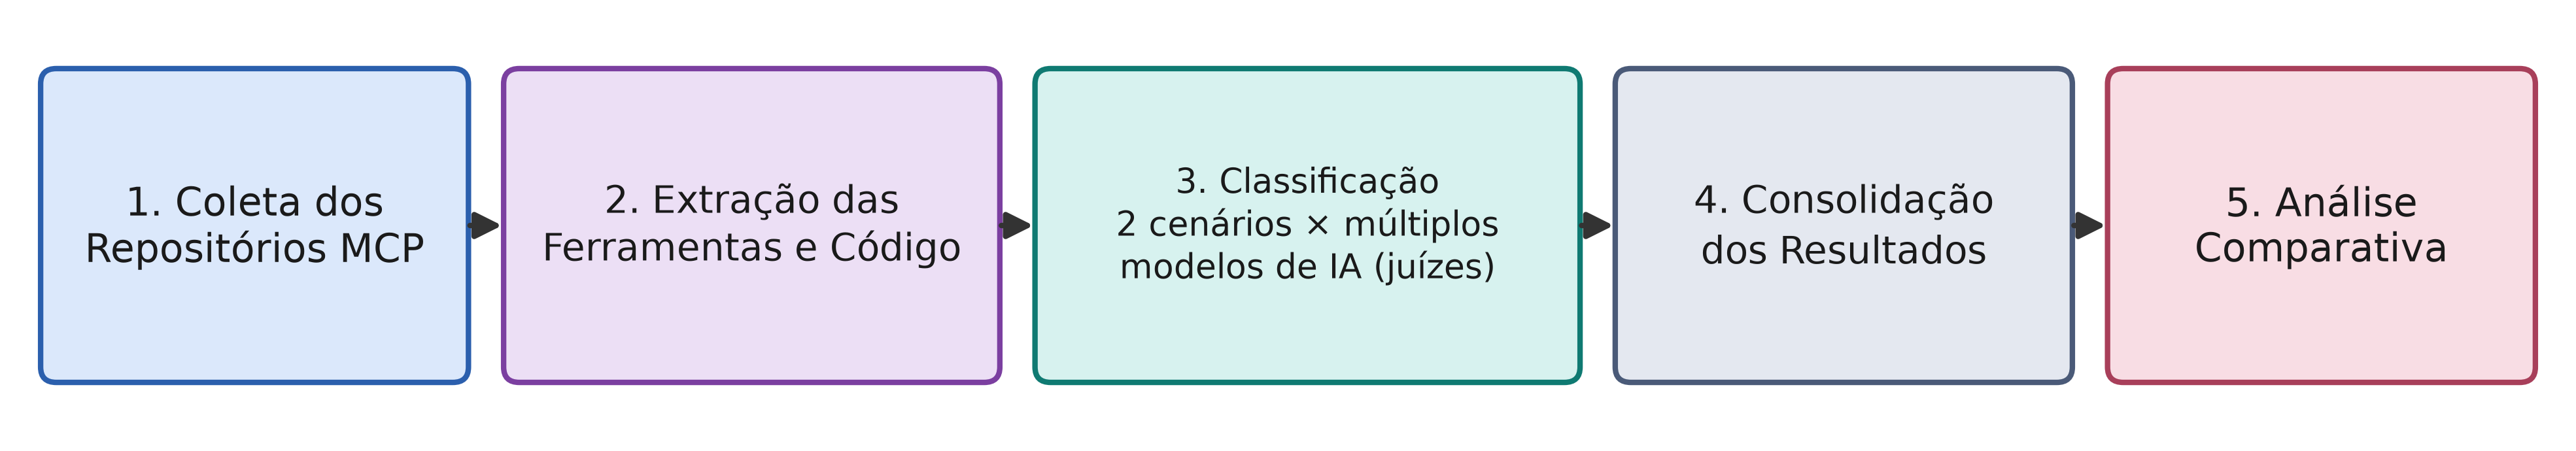
\includegraphics[width=1\linewidth]{./images/metodologia_v7.png}
    \caption{Fluxo metodológico adotado na pesquisa}
    \label{fig:metodologia}
\end{figure}

\subsection{Coleta dos Repositórios MCP}
\label{subsec:coleta}

A primeira etapa consiste na construção do conjunto de dados que \textcolor{orange}{serve} de base para os experimentos. Para isso, foram minerados repositórios públicos relacionados ao ecossistema MCP hospedados no GitHub. O objetivo dessa etapa é identificar implementações reais de servidores MCP que representem o cenário atual.

\textcolor{blue} {As consultas foram construídas a partir dos nomes dos pacotes necessários para a implementação do MCP. Para cada pacote, seu nome foi utilizado como termo de busca nos arquivos de dependências dos projetos. Essa etapa foi realizada por meio da busca de código da API REST do GitHub, que permite localizar repositórios com base em termos presentes no conteúdo de seus arquivos, ainda que a API limite cada consulta a um máximo de 1.000 resultados \cite{BashInTheWild}. Dessa forma, foi necessário dividir a busca em consultas distintas, a fim de ampliar a quantidade de projetos identificáveis. Para isso, foi realizada uma consulta para cada combinação entre o nome da dependência e o respectivo arquivo de dependências em que ela poderia estar declarada. Como essa busca de código não devolve metadados do repositório em si, cada resultado foi complementado por uma consulta separada à API GraphQL do GitHub, de onde vieram o número de estrelas, a condição de \textit{fork} e a linguagem principal usados nos filtros seguintes. Ao final, os repositórios duplicados foram unificados por identificador. Após isto, os que eram \textit{fork} e os que não atingiam o piso mínimo de estrelas, ou cuja linguagem principal não estava entre as linguagens-alvo do estudo, foram removidos.}

Para garantir a relevância e a maturidade dos \textit{softwares} analisados, a coleta foi restrita a repositórios que possuam no mínimo 100 estrelas (\textit{stars}). A adoção desse limiar fundamenta-se em estudos de mineração de repositórios que identificam o número de estrelas como uma medida direta de popularidade, sendo 100 estrelas um marco estatístico comum para filtrar projetos experimentais ou de baixo valor agregado, conhecidos como \textit{toy repositories} \cite{Borges2016}. Ao final, foram selecionados os 206 servidores mais populares encontrados e que possuíam ao menos uma tool, dobrando a amostra utilizada no estudo de Hasan et al. (2026)\nocite{2026arXiv260214878M} para ampliar a cobertura do ecossistema investigado.

\textcolor{orange}{A Figura \ref{fig:fluxo-etapa1} detalha o funcionamento interno dessa etapa. A mineração é realizada via API REST de busca de código do GitHub, segmentada por termos: cada combinação entre um sinal de dependência (por exemplo, \texttt{@modelcontextprotocol/sdk}) e um arquivo de manifesto onde esse sinal poderia estar declarado (por exemplo, \texttt{package.json}) gera uma sub-consulta independente; a linguagem não faz parte dessa segmentação e só é determinada depois, na hidratação de cada candidato. Cada repositório encontrado é então hidratado via GraphQL para a obtenção de seus metadados de linguagem principal e número de estrelas, informações não disponíveis diretamente na busca de código. Em seguida, os repositórios são unificados por identificador (removendo duplicatas encontradas por mais de uma sub-consulta) e submetidos à verificação de elegibilidade descrita acima. Os repositórios aprovados são ordenados por número de estrelas, e os mais relevantes são extraídos para compor a amostra final.}

\begin{figure}[H]
    \centering
    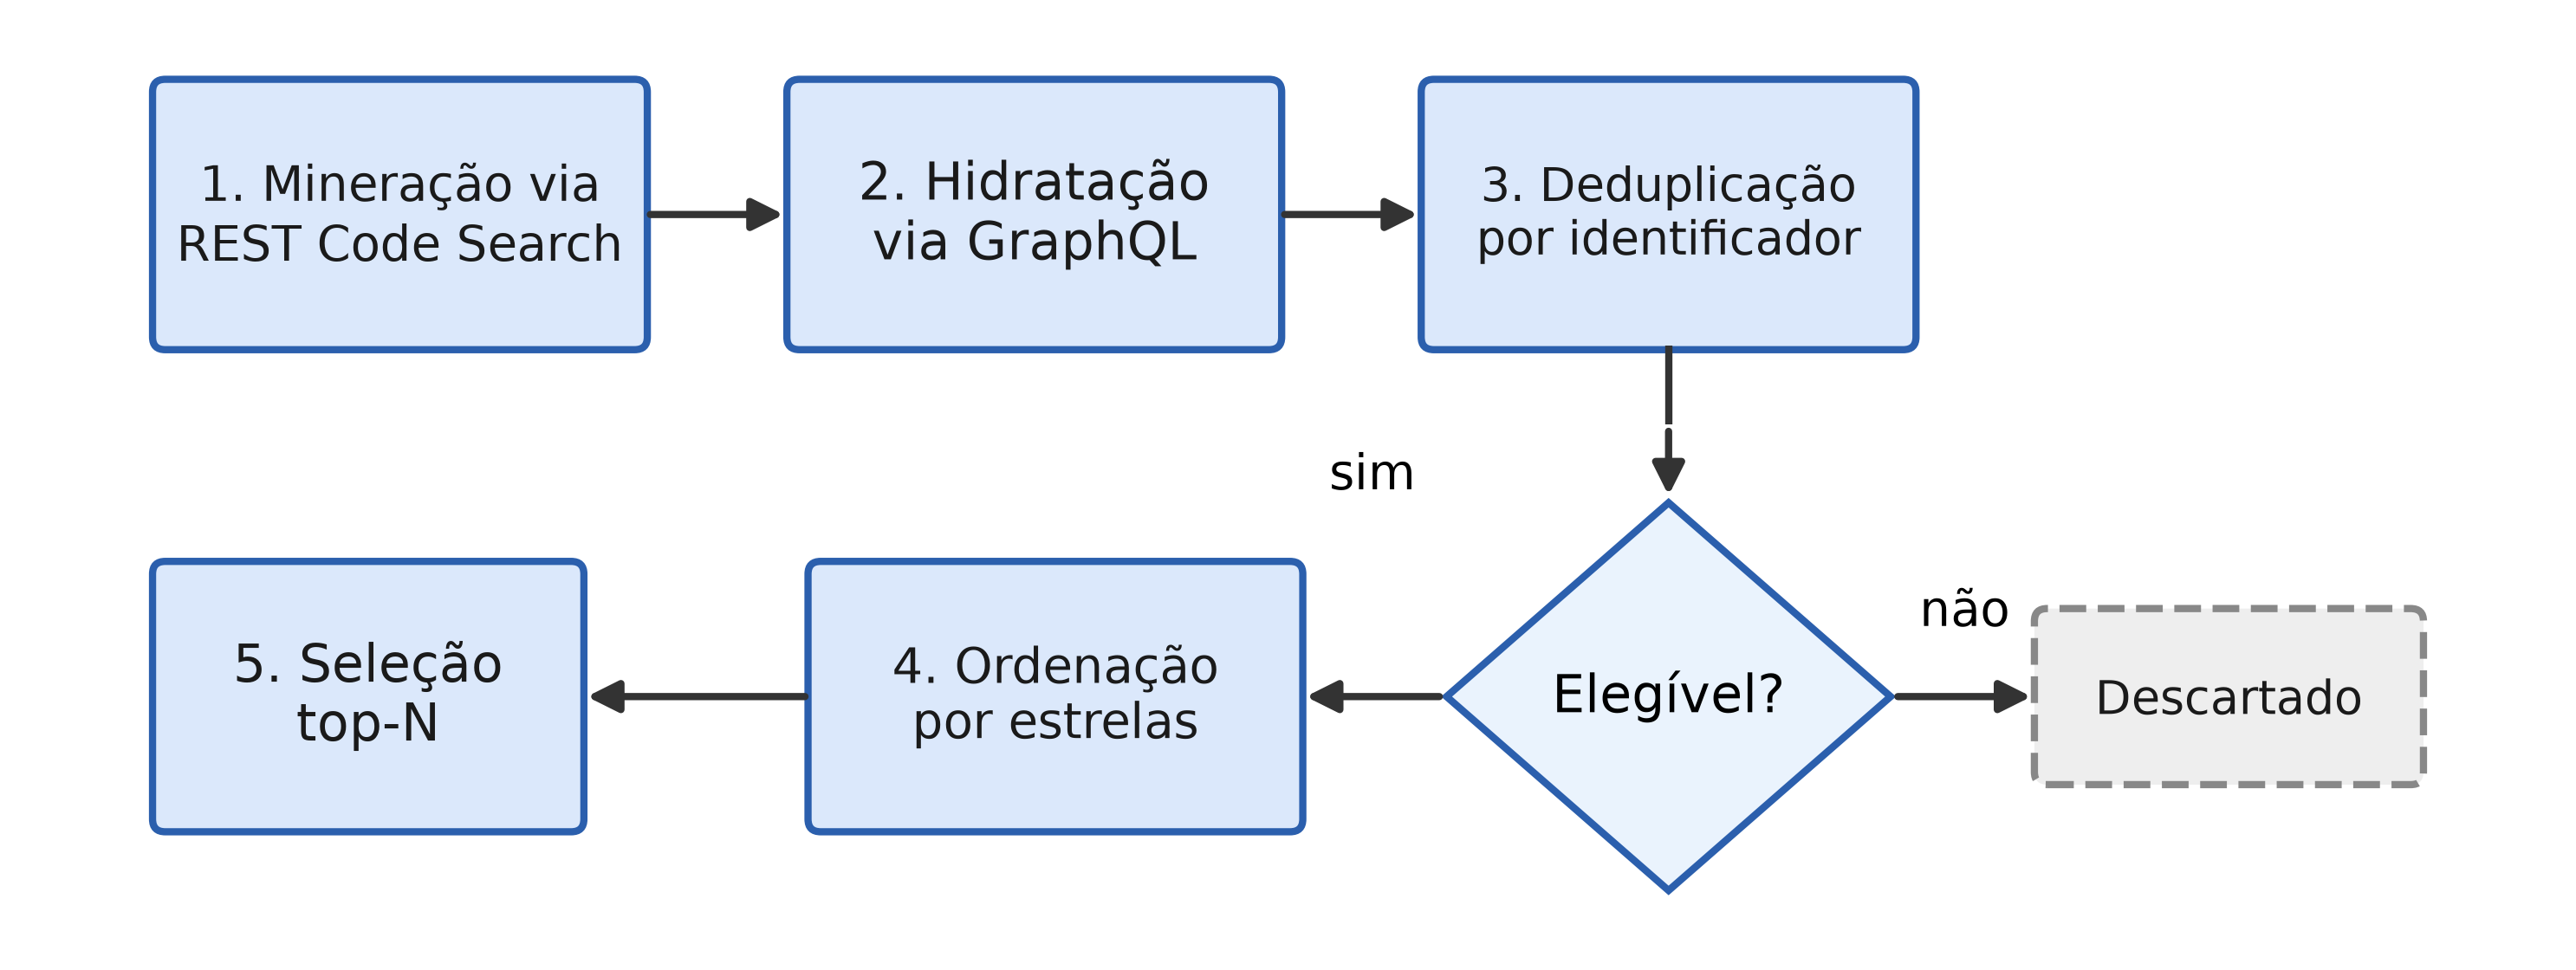
\includegraphics[width=1\linewidth]{./images/fluxo_etapa1_detalhado.png}
    \caption{Funcionamento detalhado da Etapa 1 (Coleta dos Repositórios)}
    \label{fig:fluxo-etapa1}
\end{figure}

\textcolor{orange}{A busca por sinais de manifesto devolveu 12.058 candidatos brutos, todos provenientes de arquivos de dependência (\texttt{package.json}, \texttt{pyproject.toml}, \texttt{pom.xml} e equivalentes), únicos após a deduplicação por identificador. A Tabela \ref{tab:funil-coleta} apresenta o funil de atrito aplicado sobre esse conjunto: o filtro de elegibilidade (repositório não ser \textit{fork}, possuir pelo menos 100 estrelas e estar em uma das linguagens-alvo) reduziu esse conjunto para 723 repositórios.}

\begin{table}[H]
\centering
\caption{Funil de atrito da Etapa 1 (Coleta dos Repositórios MCP)}
\label{tab:funil-coleta}
\begin{tabular}{|p{0.6\linewidth}|r|r|}
\hline
\textbf{Etapa do filtro} & \textbf{Repositórios} & \textbf{\% do bruto} \\ \hline
Candidatos brutos (busca por manifesto) & 12.058 & 100,0\% \\ \hline
Aprovados no filtro (não-fork, estrelas $\geq$ mínimo, linguagem-alvo) & 723 & 6,0\% \\ \hline
Selecionados (qualificados pelo laço de \textit{backfill}) & 206 & 1,7\% \\ \hline
\end{tabular}
\end{table}

\textcolor{orange}{Diferentemente de um corte simples pelas 206 posições mais bem colocadas, a seleção final passa por um laço de preenchimento (\textit{backfill}): um repositório só permanece selecionado se, após a Etapa 2, confirmar pelo menos uma ferramenta; repositórios desqualificados são substituídos pelo próximo candidato do pool ainda não tentado, e o processo se repete até fechar as 206 vagas ou esgotar o pool. Entre os repositórios selecionados, a distribuição por linguagem principal está longe de ser uniforme (Figura \ref{fig:repos-linguagem}).}

\begin{figure}[H]
    \centering
    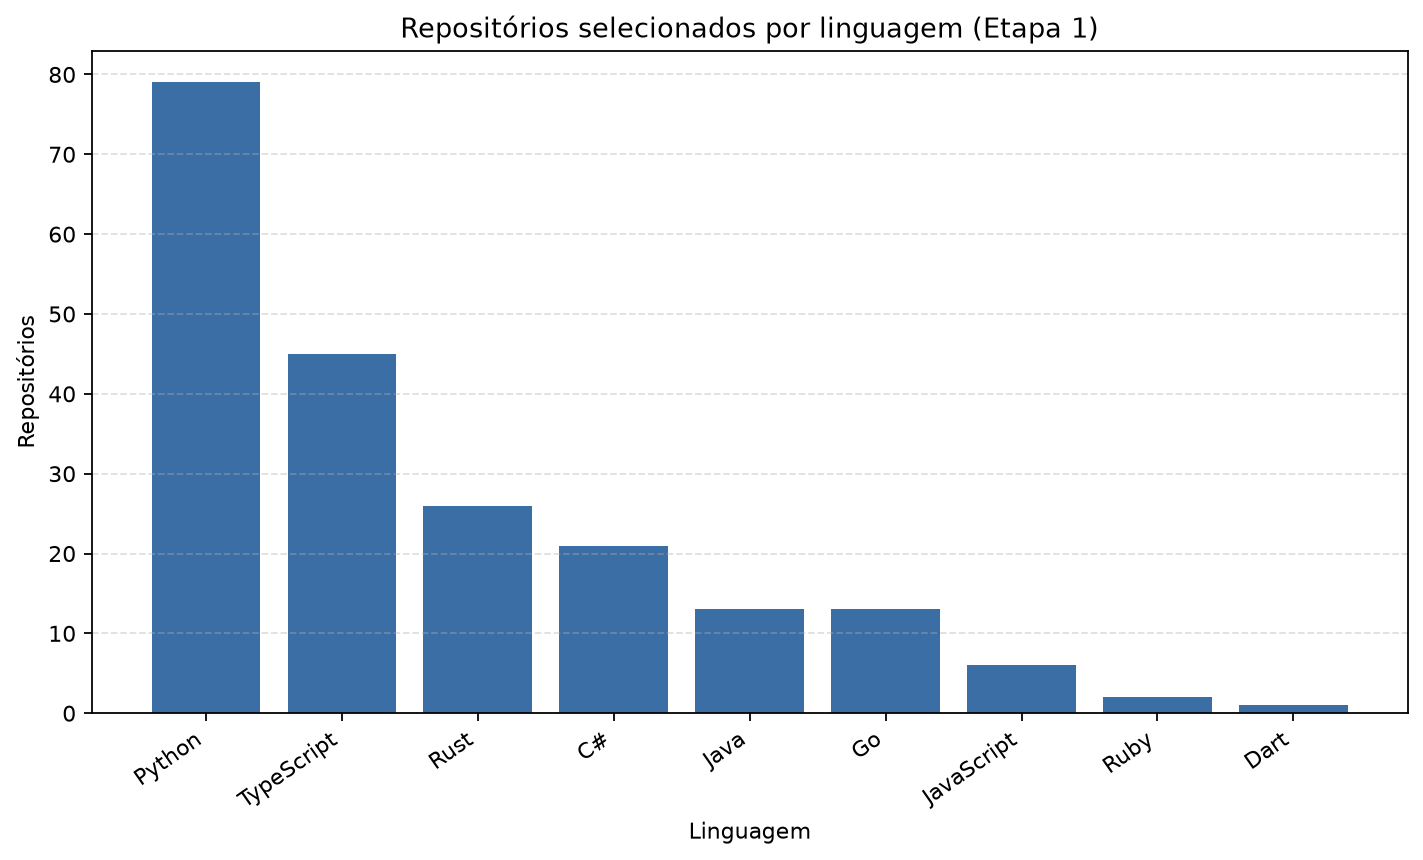
\includegraphics[width=0.8\linewidth]{./images/01_repos_por_linguagem.png}
    \caption{Repositórios selecionados por linguagem principal (Etapa 1)}
    \label{fig:repos-linguagem}
\end{figure}

\textcolor{orange}{Python (79, 38,3\%) e TypeScript (45, 21,8\%) concentram 60\% da amostra, seguidos por Rust (26), C\# (21), Java e Go (13 cada); JavaScript, Ruby e Dart somam, juntos, o restante. Nenhum repositório em Kotlin, PHP, Elixir, Lua ou Swift permaneceu na seleção final: os candidatos dessas linguagens que chegaram a ser selecionados foram descartados pelo laço de \textit{backfill} por não confirmarem nenhuma ferramenta na Etapa 2 (Seção~\ref{subsec:extracao}), ou nunca alcançaram o piso de estrelas dentro do pool.}


\subsection{Extração das Ferramentas e do Código Relacionado}
\label{subsec:extracao}

Após a obtenção dos repositórios, cada um foi clonado localmente para permitir a identificação automática das ferramentas
disponibilizadas por cada servidor MCP, chegando ao resultado de 12.171
ferramentas. Para isso, foi desenvolvido um algoritmo de mineração capaz
de percorrer a estrutura dos projetos e localizar as implementações
associadas às ferramentas expostas pelo servidor. Para cada ferramenta
identificada, foram extraídos sua descrição em linguagem natural e sua
localização no código. Um repositório em que nenhuma ferramenta é
localizada é tratado, na prática, como um falso positivo da etapa de
coleta: ele é removido da amostra e substituído pelo próximo candidato
ainda não testado, repetindo-se o processo até completar o número de
repositórios definido para o estudo ou esgotar os candidatos disponíveis\textcolor{orange}{, fechando o mesmo laço de \textit{backfill} descrito na Seção~\ref{subsec:coleta}}.

\textcolor{orange}{A Figura \ref{fig:fluxo-etapa2} detalha o funcionamento interno dessa etapa (clonagem, detecção de ferramentas e construção do grafo de chamadas), incluindo o laço de \textit{backfill} entre Etapas 1 e 2. Cada repositório selecionado é primeiro clonado e então indexado estaticamente: são catalogadas todas as definições de função/método e, por arquivo, os \textit{imports} declarados. Em seguida, aplica-se o padrão estrutural do SDK correspondente à linguagem do repositório para localizar as ferramentas declaradas; se nenhuma ferramenta é encontrada, o repositório é desqualificado e substituído, reentrando no fluxo a partir da clonagem.}

\begin{figure}[H]
    \centering
    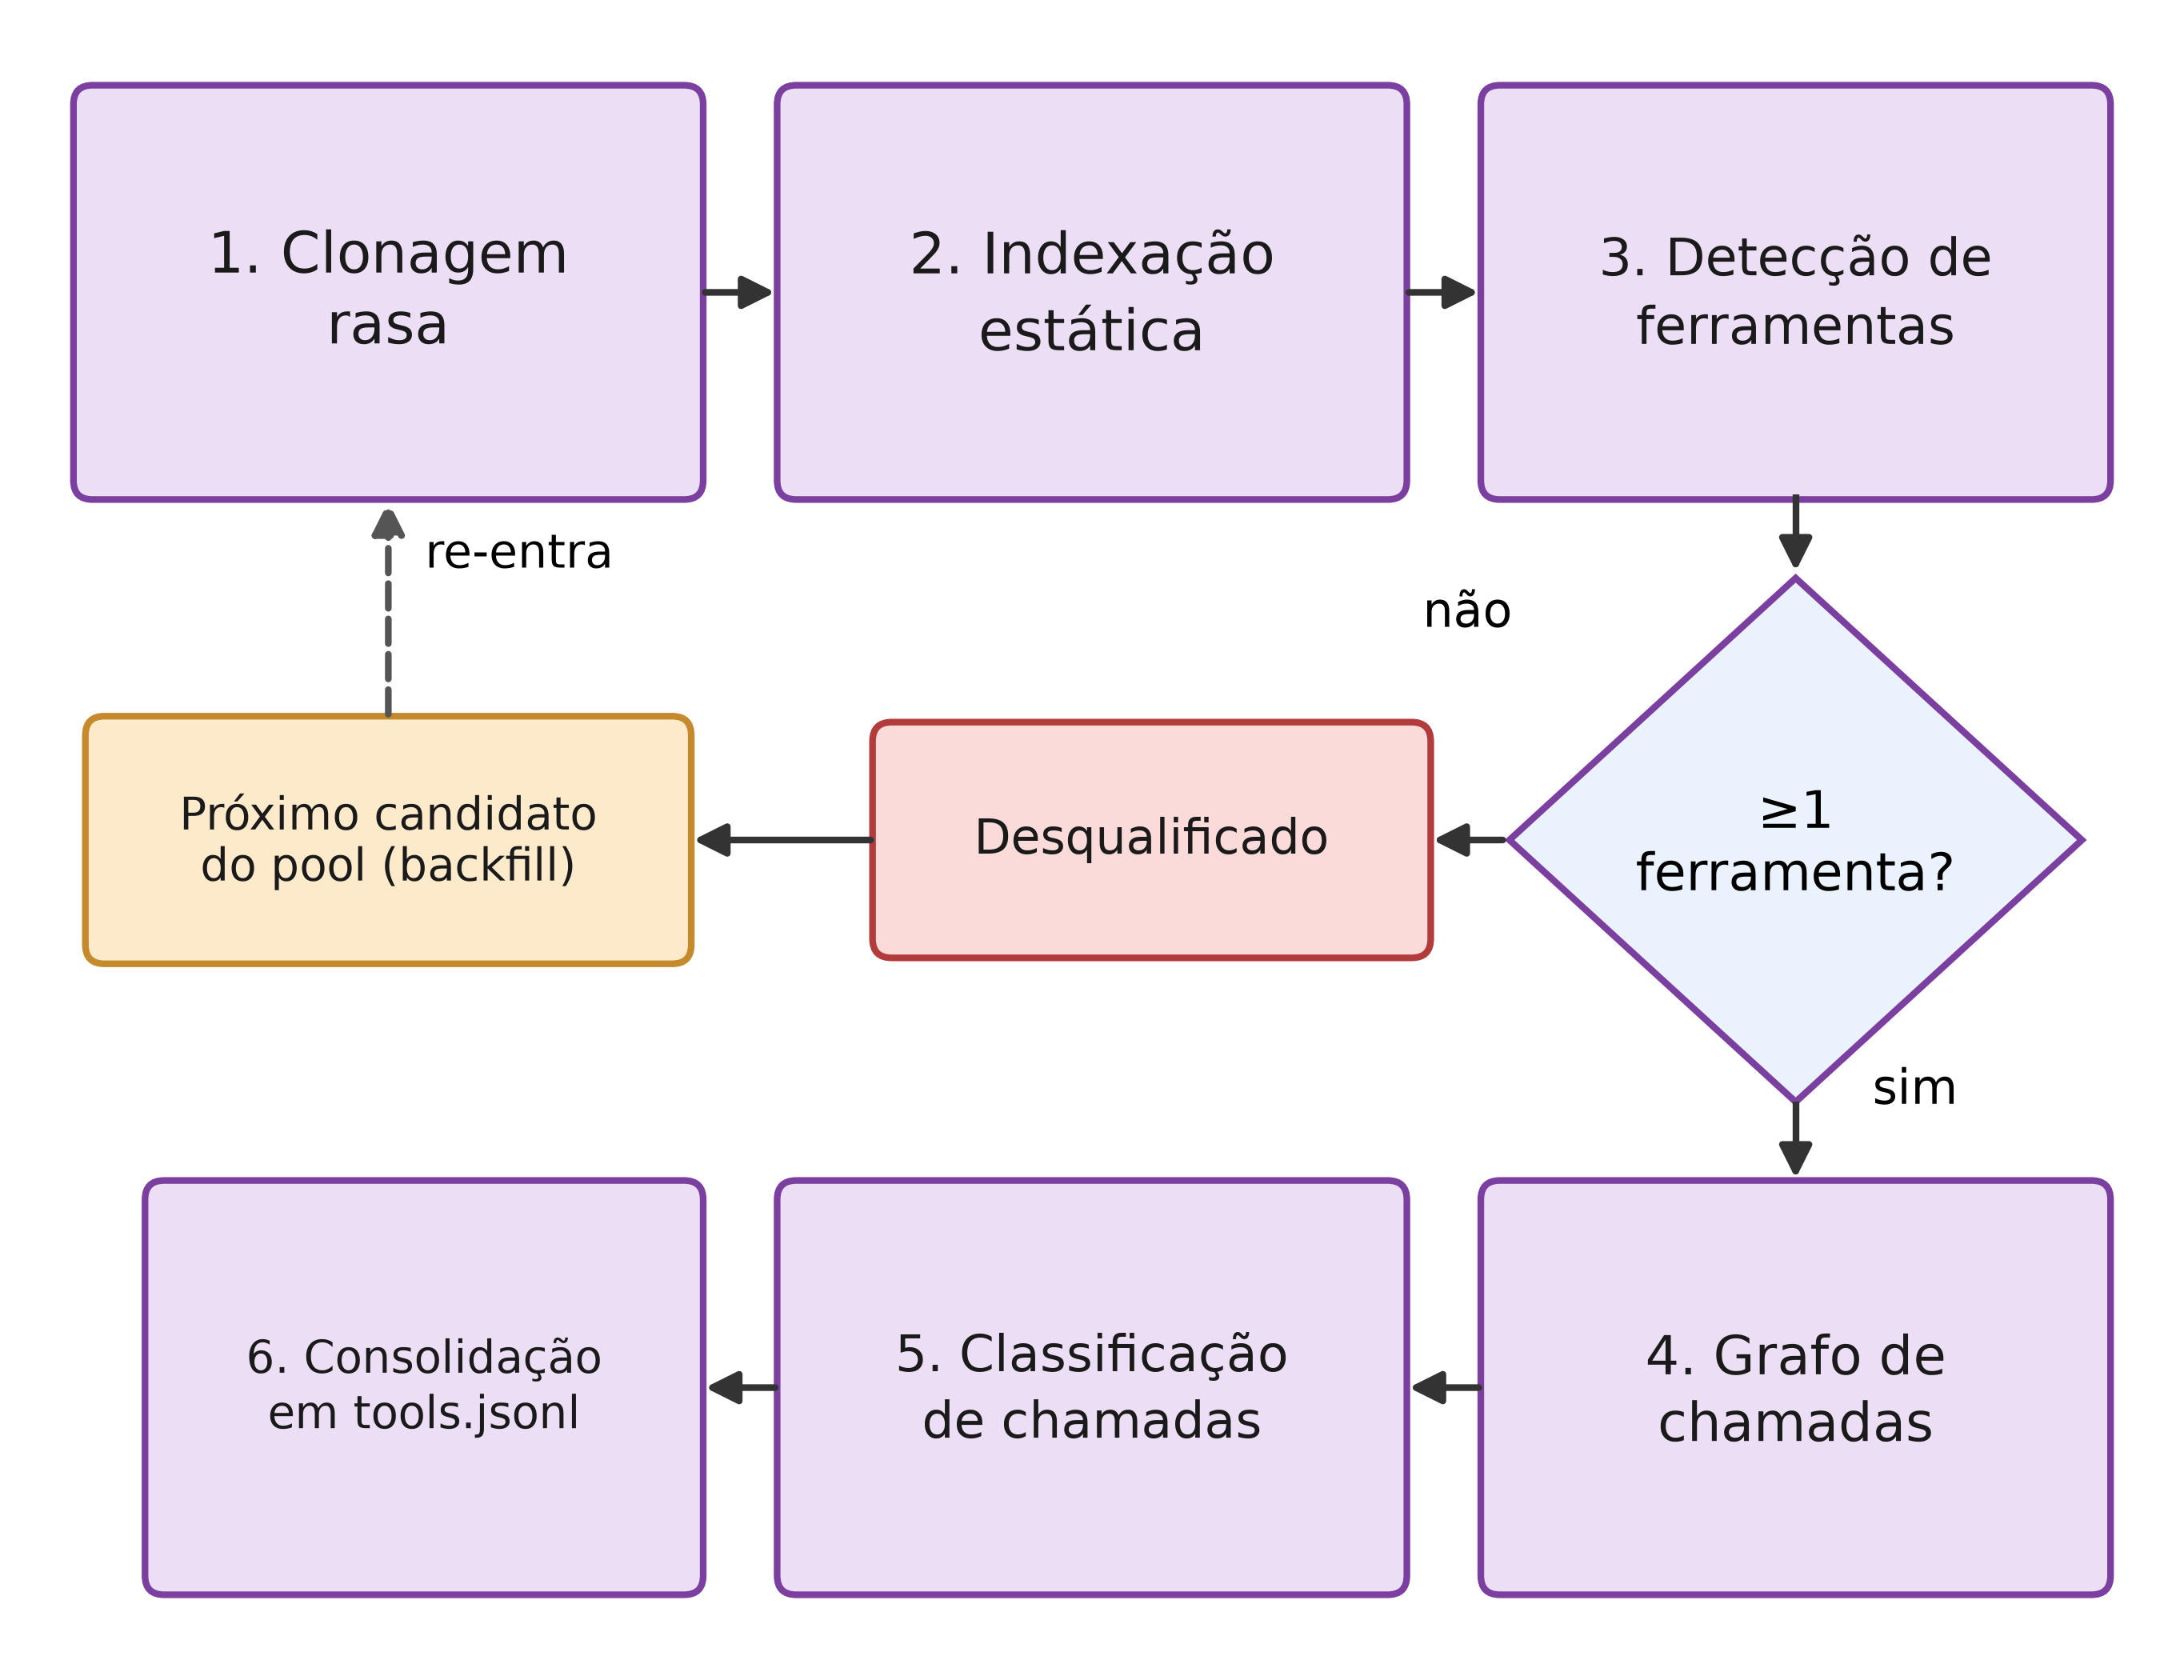
\includegraphics[width=1\linewidth]{./images/fluxo_etapa2_detalhado.png}
    \caption{Funcionamento detalhado da Etapa 2 (Extração das Ferramentas)}
    \label{fig:fluxo-etapa2}
\end{figure}

Em seguida, foi realizada a extração do código relacionado a cada ferramenta. Como os servidores MCP possuem estruturas variadas, extrair apenas o método raiz de uma ferramenta pode não ser suficiente para capturar sua lógica, sendo necessário incluir também os métodos subsequentemente invocados. Para isso, foi construída uma árvore de chamadas (\textit{call graph}) a partir do método inicial\textcolor{orange}{, expandida recursivamente até um limite máximo de três níveis de profundidade}: o próprio método inicial constitui o primeiro nível; os métodos chamados diretamente por ele\textcolor{orange}{, quando resolvidos,} formam o segundo nível; e as chamadas efetuadas a partir destes compõem o terceiro nível. \textcolor{orange}{A limitação da profundidade a três níveis é uma decisão de engenharia, não uma medição prévia de onde termina a lógica relevante de uma ferramenta: ela contém o custo da análise (e do texto eventualmente enviado ao avaliador) e elimina, por construção, qualquer risco de recursão infinita, sem exigir detecção de ciclo separada (ver Apêndice~\ref{apendice:secao} para o detalhamento completo da heurística de resolução).} Um exemplo desse processo é apresentado na Figura \ref{fig:codigoarvore}.

\begin{figure}[H]
    \centering
    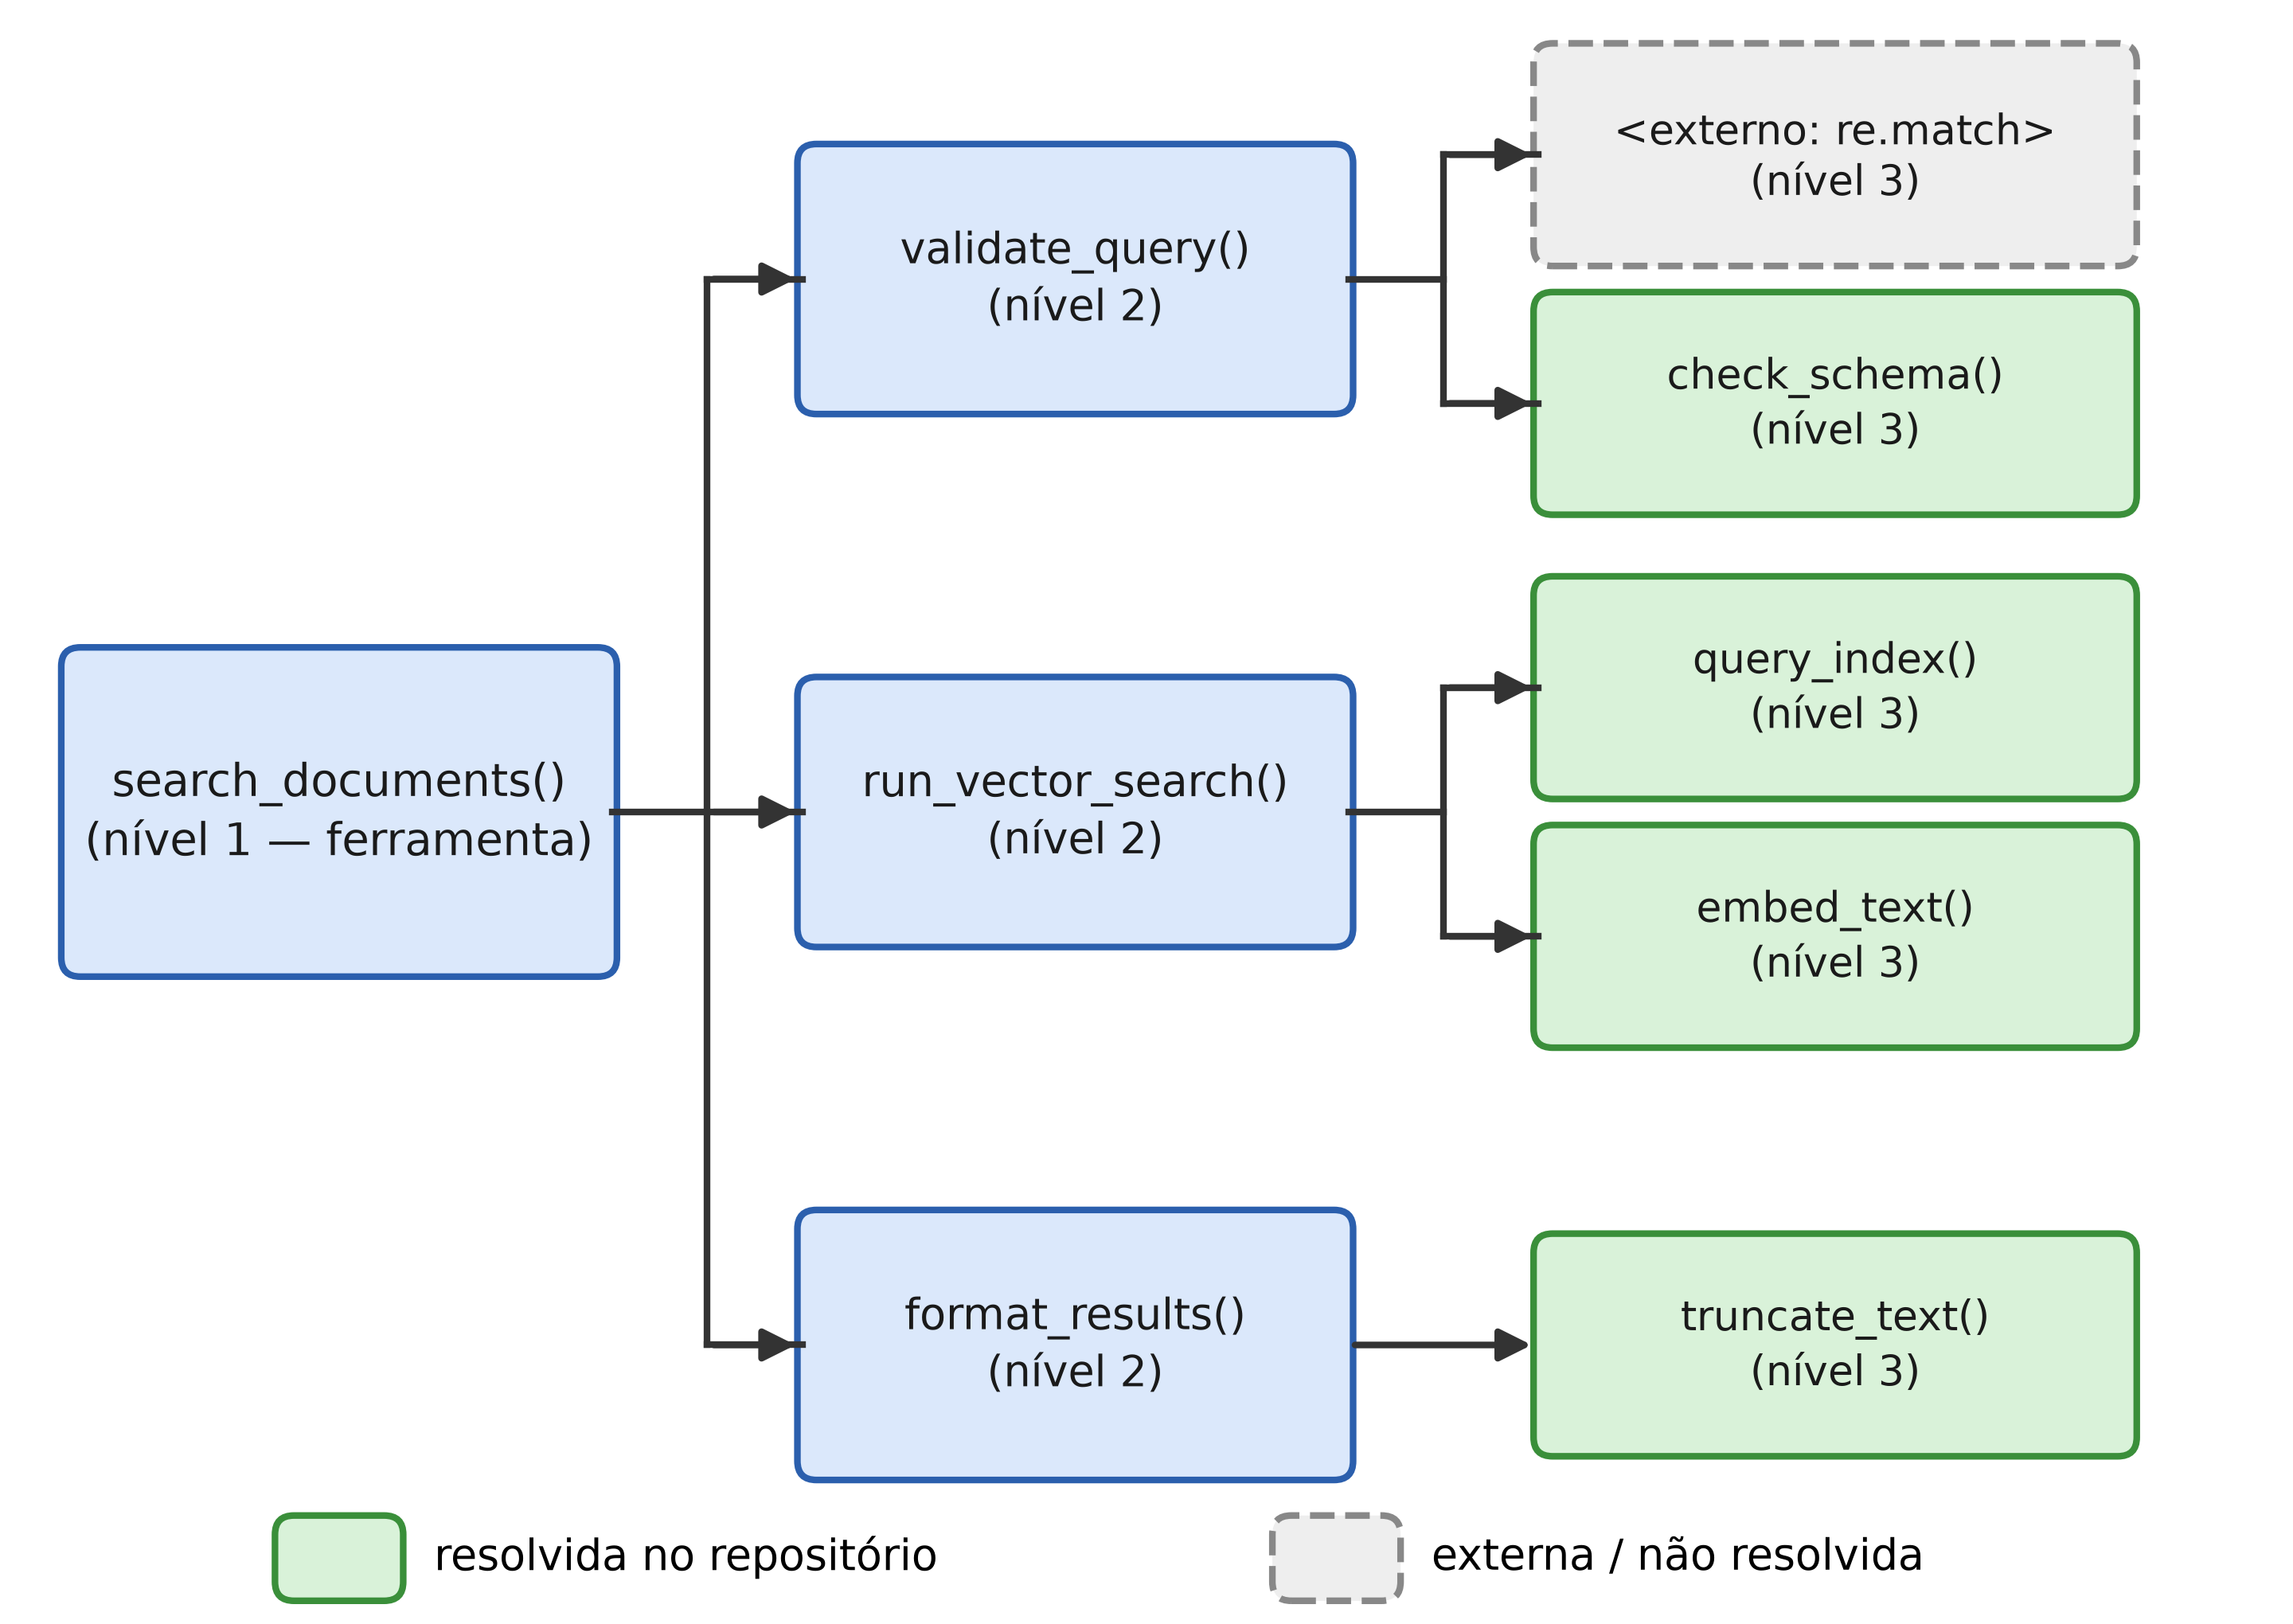
\includegraphics[width=1\linewidth]{./images/arvoreFinal.png}
    \caption{Exemplo de extração da árvore de chamadas de uma ferramenta}
    \label{fig:codigoarvore}
\end{figure}

Ao final desta etapa, foi produzido um conjunto de dados estruturado contendo os servidores MCP analisados e as ferramentas identificadas em cada um deles. Para cada ferramenta, \textcolor{orange}{são armazenadas} sua descrição em linguagem natural e o conjunto de métodos obtido a partir da árvore de chamadas. Esse conjunto de dados \textcolor{orange}{serve} como entrada para as etapas subsequentes da pesquisa, nas quais as ferramentas dos repositórios coletados \textcolor{orange}{são avaliadas} quanto à qualidade de suas descrições, com e sem o uso do código correspondente.

\textcolor{orange}{A Etapa 2 extraiu 12.171 ferramentas dos 206 repositórios selecionados; como a seleção final já incorpora o laço de \textit{backfill}, todo repositório selecionado confirma, por construção, pelo menos uma ferramenta. A distribuição de ferramentas por linguagem (Figura~\ref{fig:tools-linguagem}) segue de perto a distribuição de repositórios vista na coleta.}

\begin{figure}[H]
    \centering
    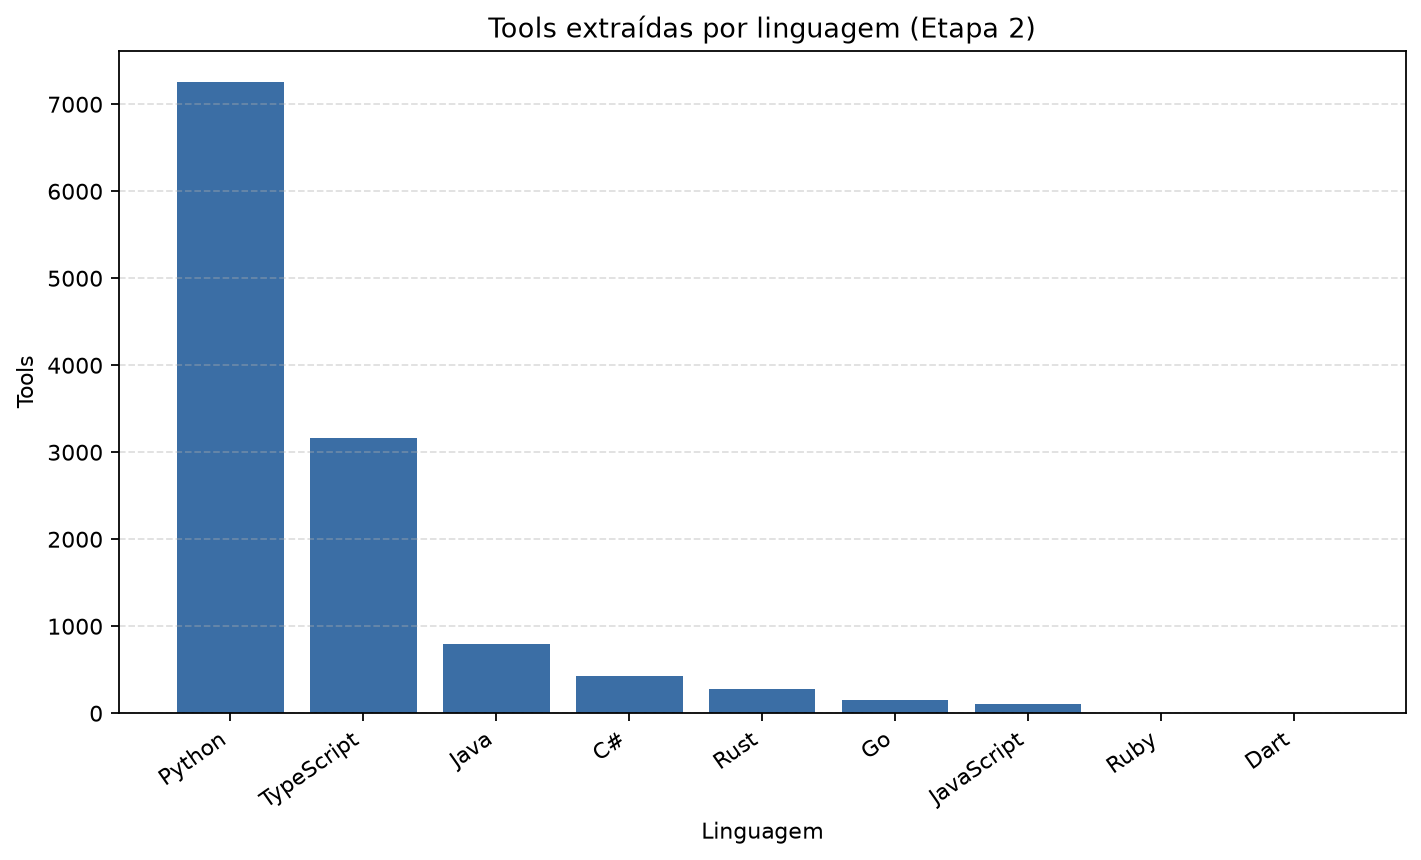
\includegraphics[width=0.8\linewidth]{./images/02_tools_por_linguagem.png}
    \caption{Ferramentas extraídas por linguagem (Etapa 2)}
    \label{fig:tools-linguagem}
\end{figure}

\textcolor{orange}{Python concentra 7.251 das 12.171 ferramentas (59,6\%), seguido por TypeScript (3.162, 26,0\%) e Java (793, 6,5\%); as demais linguagens somam, juntas, pouco mais de 7\% do total (Tabela~\ref{tab:media-tools-servidor}).}

\begin{table}[H]
\centering
\caption{Repositórios selecionados e total de ferramentas extraídas, por linguagem}
\label{tab:media-tools-servidor}
\begin{tabular}{|l|r|r|r|}
\hline
\textbf{Linguagem} & \textbf{Repositórios} & \textbf{Tools (total)} & \textbf{Média/repositório} \\ \hline
Python & 79 & 7.251 & 91,78 \\ \hline
TypeScript & 45 & 3.162 & 70,27 \\ \hline
Java & 13 & 793 & 61,00 \\ \hline
C\# & 21 & 423 & 20,14 \\ \hline
Rust & 26 & 276 & 10,62 \\ \hline
Go & 13 & 149 & 11,46 \\ \hline
JavaScript & 6 & 108 & 18,00 \\ \hline
Ruby & 2 & 5 & 2,50 \\ \hline
Dart & 1 & 4 & 4,00 \\ \hline
\textbf{Total} & \textbf{206} & \textbf{12.171} & \textbf{59,08} \\ \hline
\end{tabular}
\end{table}

\textcolor{orange}{A concentração de ferramentas por repositório também é fortemente assimétrica: os três repositórios com mais ferramentas respondem, sozinhos, por 46,6\% de todo o conjunto de dados (20,4\%, 18,4\% e 7,8\%, respectivamente), um deles em TypeScript, os outros dois em Python. Esse resultado eleva consideravelmente a média de ferramentas por repositório nessas duas linguagens (Tabela~\ref{tab:media-tools-servidor}) e deve ser considerado ao interpretar médias agregadas por linguagem.}

REESCREVER ESTE PARAGRAFO\textcolor{orange}{Quanto ao grafo de chamadas construído para cada ferramenta, 30,9\% das chamadas (entre os níveis 2 e 3) foram resolvidas sem ambiguidade dentro do próprio repositório, 11,0\% foram resolvidas por desempate entre candidatos ambíguos, e 58,1\% permaneceram como chamadas externas ou dinamicamente determinadas — resultado consistente com o fato de que boa parte da lógica invocada por uma ferramenta MCP reside em bibliotecas de terceiros ou na biblioteca padrão da linguagem, fora do escopo de resolução do algoritmo (ver Apêndice~\ref{apendice:secao}).}


\subsection{Classificação das tools por diferentes modelos de IA}

Na terceira etapa, utilizando as \textit{tools} coletadas nas etapas anteriores, \textcolor{orange}{é conduzido} um experimento comparativo estruturado em dois cenários de avaliação\textcolor{orange}{, executados} em diferentes modelos de IA. No primeiro cenário, as descrições das ferramentas \textcolor{orange}{são avaliadas} com base em seu conteúdo em linguagem natural. No segundo, essas mesmas descrições \textcolor{orange}{são avaliadas} em conjunto com informações extraídas do código correspondente. Essa estratégia permite identificar o impacto da inclusão do contexto de implementação na avaliação da qualidade das descrições.

\textcolor{orange}{A Figura \ref{fig:fluxo-etapa3} detalha o funcionamento interno dessa etapa. Para cada ferramenta, são montados os dois cenários de avaliação descritos acima; cada cenário gera um \textit{payload} contendo o nome da ferramenta, seu servidor de origem, a descrição e, quando aplicável, o código de contexto, enviado a cada juiz habilitado de forma concorrente. As respostas dos juízes podem resultar em uma avaliação concluída, em uma recusa de segurança do provedor, ou em um erro técnico durante o processamento. As duas primeiras são gravadas no arquivo de resultados e recebem uma entrada de \textit{checkpoint}, permitindo retomar a execução sem repetir avaliações já concluídas; o erro técnico não gera registro de resultado nem entrada de \textit{checkpoint}, apenas um registro em um log de erros separado, e é reprocessado automaticamente na rodada seguinte.}

\begin{figure}[H]
    \centering
    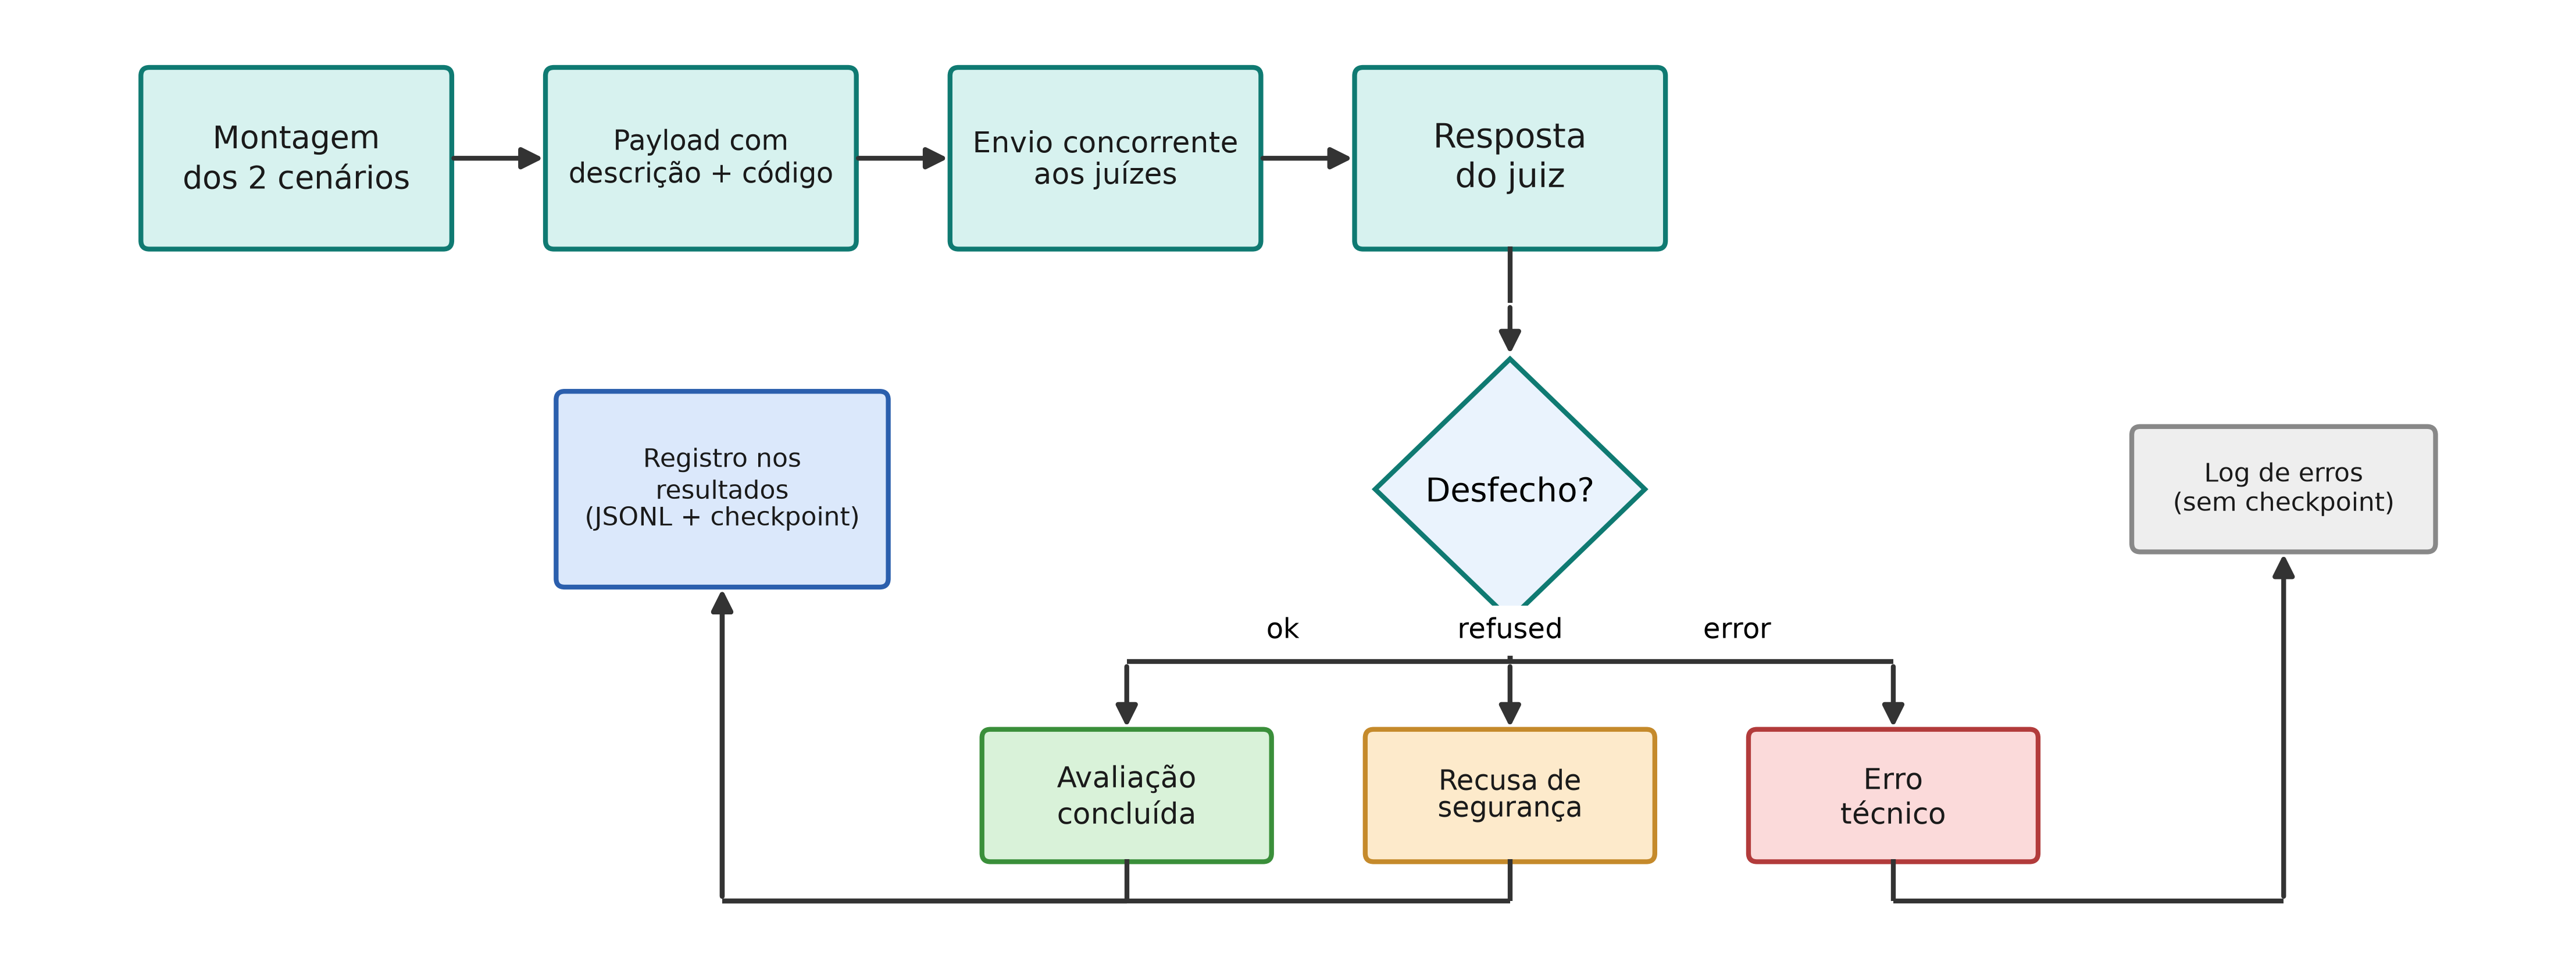
\includegraphics[width=1\linewidth]{./images/fluxo_etapa3_detalhado.png}
    \caption{Funcionamento detalhado da Etapa 3 (Classificação das Ferramentas)}
    \label{fig:fluxo-etapa3}
\end{figure}

Em ambos os cenários, a avaliação \textcolor{orange}{é conduzida} com base na rubrica proposta por Hasan et al. (2026)\nocite{2026arXiv260214878M}, composta por seis componentes: \textit{Purpose}, que avalia a clareza com que a descrição comunica a finalidade da ferramenta; \textit{Guidelines}, que verifica se existem orientações sobre quando e como utilizá-la; \textit{Limitations}, que analisa a explicitação de restrições, premissas ou casos de falha; \textit{Parameter Explanation}, que mede a qualidade da documentação dos parâmetros de entrada; \textit{Length and Completeness}, que avalia o nível de detalhamento e cobertura da descrição; e \textit{Examples}, que verifica a presença de exemplos de utilização. Cada componente recebe uma pontuação em uma escala Likert de cinco pontos, sendo posteriormente utilizada para identificar deficiências associadas aos respectivos \textit{smells} descritos pelos autores.

\textcolor{orange}{Em ambos os cenários, os modelos de linguagem atuam como o mesmo avaliador (\textit{LLM-as-a-Judge}), recebendo as descrições das ferramentas e atribuindo as seis pontuações da rubrica acima.} No primeiro cenário\textcolor{orange}{, essa avaliação} é realizada sem qualquer acesso à implementação da funcionalidade analisada. No segundo cenário, \textcolor{orange}{o mesmo avaliador recebe adicionalmente} o código correspondente, \textcolor{orange}{ isto é, os trechos de código-fonte reunidos pela árvore de chamadas construída na Seção~\ref{subsec:extracao}}. Dessa forma, o avaliador \textcolor{orange}{pode} confrontar a descrição fornecida com aspectos observáveis da implementação, verificando a existência de omissões, inconsistências ou informações potencialmente enganosas que não seriam perceptíveis apenas pela análise da descrição.


\subsection{\textcolor{orange}{Consolidação dos Resultados por Cenário}}

Concluída a etapa de classificação, os resultados produzidos nos dois cenários experimentais \textcolor{orange}{são coletados e estruturados} em uma base de dados unificada. Para cada ferramenta analisada, \textcolor{orange}{são armazenados} identificadores que \textcolor{orange}{permitem} sua associação ao servidor MCP de origem, bem como os resultados obtidos nos cenários com e sem a inclusão de informações provenientes do código, além de qual modelo de IA foi utilizado na avaliação.

A base de dados resultante \textcolor{orange}{contém} os escores atribuídos pelo modelo para cada dimensão de qualidade avaliada, além das classificações finais produzidas em cada execução do experimento. Dessa forma, cada ferramenta \textcolor{orange}{possui} dois conjuntos de resultados por modelo\textcolor{orange}{, diretamente vinculados} à mesma descrição, diferindo apenas pela presença ou ausência das informações extraídas do código. Essa organização \textcolor{orange}{estabelece} um relacionamento direto entre as avaliações realizadas sobre uma mesma ferramenta, preservando o pareamento necessário para as análises estatísticas subsequentes e possibilitando a comparação consistente dos resultados obtidos nos dois cenários experimentais.


\subsection{Análise Comparativa dos Experimentos}

Na etapa final, os resultados obtidos \textcolor{orange}{são analisados} com o objetivo de identificar diferenças entre os dois cenários de avaliação. Essa análise busca validar se a utilização do código de fato altera os resultados da avaliação das descrições, além de identificar quais atributos da rubrica utilizada para avaliar a qualidade são mais e menos impactados pela adição do código.

Inicialmente, \textcolor{orange}{realiza-se} uma análise por meio do cálculo de medidas como média, mediana e desvio-padrão dos escores atribuídos a cada dimensão de qualidade avaliada, para identificar se \textcolor{orange}{há} diferença numérica nos resultados gerados com e sem o contexto do código das ferramentas MCP, atendendo ao objetivo específico (ii) desta pesquisa. A partir dessa comparação, é possível avaliar quais atributos \textcolor{orange}{são} mais afetados pela inserção do contexto técnico. \textcolor{orange}{Aplica-se} também o Teste de Postos Sinalizados de Wilcoxon \cite{wilcoxon1945individual}, \textcolor{orange}{individualmente} para cada dimensão de qualidade, a fim de verificar se as diferenças observadas entre as avaliações são estatisticamente significativas, concluindo o objetivo específico (iii). O teste \textcolor{orange}{é aplicado} separadamente para cada modelo de linguagem utilizado, permitindo verificar se o efeito da inclusão do código se mantém consistente entre diferentes avaliadores. Como as duas avaliações são realizadas sobre a mesma ferramenta, o teste é adequado por considerar amostras pareadas e não exigir a suposição de normalidade dos dados. Os resultados dessa análise \textcolor{orange}{fornecem} as evidências empíricas necessárias para apoiar ou refutar a hipótese de que a incorporação do contexto técnico amplia a capacidade de detecção de \textit{smells} em descrições de ferramentas MCP.

\textcolor{orange}{Formalmente, para cada dimensão da rubrica e cada juiz, testa-se a hipótese nula de que a distribuição das diferenças pareadas entre os escores dos cenários \texttt{with\_source} e \texttt{description\_only} é simétrica em torno de zero, contra a hipótese alternativa de que a inclusão do código desloca essa distribuição. Como o teste é repetido para as seis dimensões da rubrica em cada juiz, \textcolor{orange}{avalia-se} a necessidade de correção para comparações múltiplas antes de reportar significância. Pares de ferramentas em que os dois cenários recebem exatamente o mesmo escore (diferença zero) são descartados do cálculo do teste, conforme o tratamento padrão de empates do Teste de Wilcoxon; a proporção de pares descartados por esse motivo \textcolor{orange}{é reportada} junto com o resultado do teste, por dimensão, como indicador adicional do quanto a inclusão do código muda ou não a nota atribuída. Essa análise é implementada no mesmo script de análise dedicado da subseção anterior, a partir da base consolidada ali descrita.}
